\chapter{Implementacja}
\section{Wprowadzenie}
Celem tego rozdziału jest szczegółowy opis podejścia do realizacji projektu BBS, a mianowicie wyjaśnienie podstawowych pojęć, analiza architektury oraz algorytmów stosowanych do przetwarzania danych.

Chciałbym zacząć od tego, czym właściwie jest BBS. Zgodnie z definicją projekt jest w rzeczywistości procesorem języka \cite{compilers}, a konkretnie tłumaczem według następujących cech, które wynikają bezpośrednio z wymagań opisanych w sekcji 2:
\begin{itemize}
    \item Oprogramowanie analizuje kod wejściowy, napisany w specjalnie opracowanym na potrzeby projektu języku
    \item Oprogramowanie powinno wykrywać i raportować możliwe błędy logiczne lub składniowe w pliku wejściowym
    \item Zamiast tłumaczyć plik wejściowy na inny język programowania, program powinien wykonać polecenia opisane w pliku wejściowym
\end{itemize}

Dodatkowo oprogramowanie to zawiera również preprocesor. Dzieje się tak, aby plik wejściowy mógł zostać podzielony na wiele części, co umożliwi działanie mechanizmu budowania podprojektu.

\section{Struktura interpretera}
Zgodnie ze standardową strukturą kompilatorów i interpreterów, oprogramowanie BBS implementuje część frontend (czyli tę, która przeprowadza analizę) prawie w całości, natomiast backend nie zajmuje się optymalizacją ani generowaniem kodu, ponieważ wykonuje on określone instrukcje na podstawie danych wejściowych (czyli proces syntezy de facto nie zachodzi) \cite{compilers}.

Jeśli patrzyć na dane oprogramowanie ze względu na ogólnie przyjęte fazy kompilacji (które odpowiadają opisanym powyżej częściom standardowego kompilatora lub interpretera), to BBS realizuje prawie wszystkie fazy frontendu, z wyjątkiem generowania kodu pośredniego. Wynika to z niepraktyczności generowania kodu pośredniego bez znaczących opcji jego dalszego wykorzystania. Więc BBS zamiast tej fazy ma swoją, specjalną fazę - fazę wypełniania wewnętrznej struktury opisującej projekt, który ma zostać zbudowany z BBS. Sama konstrukcja, a także procesy zachodzące w tej fazie zostaną szczegółowo opisane w dalszej części.

Podejście do implementacji backendu zasadniczo różni się od standardowego: nie jest wymagane dalsze tłumaczenie kodu na inny język, nie są realizowane fazy generowania kodu w innym języku. Zamiast tego backend na podstawie informacji o projekcie dostarczonych użytkownikowi wybiera określone polecenia do kontrolowania i budowania projektów.

Schemat fazowy BBS wygląda następująco:

\begin{figure}[h]
    \caption{Schemat fazowy projektu BBS}
    \centering
    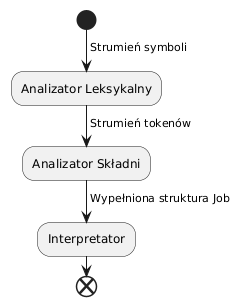
\includegraphics[width=0.4\textwidth]{Images/phases.png}
\end{figure}

Następnie opis procesu implementacji programu zostanie podzielony na części, które również dzielą się na fazy. Ma to na celu proste opisanie procesów zachodzących w środku programu, a także zademonstrowanie danych wejściowych/wyjściowych.